\documentclass{beamer}

\pdfmapfile{+sansmathaccent.map}


\mode<presentation>
{
	\usetheme{Warsaw} % or try Darmstadt, Madrid, Warsaw, Rochester, CambridgeUS, ...
	\usecolortheme{seahorse} % or try seahorse, beaver, crane, wolverine, ...
	\usefonttheme{serif}  % or try serif, structurebold, ...
	\setbeamertemplate{navigation symbols}{}
	\setbeamertemplate{caption}[numbered]
} 


%%%%%%%%%%%%%%%%%%%%%%%%%%%%
% itemize settings


%%%%%%%%%%%%%%%%%%%%%%%%%%%%
% itemize settings

\definecolor{myhotpink}{RGB}{255, 80, 200}
\definecolor{mywarmpink}{RGB}{255, 60, 160}
\definecolor{mylightpink}{RGB}{255, 80, 200}
\definecolor{mypink}{RGB}{255, 30, 80}
\definecolor{mydarkpink}{RGB}{155, 25, 60}

\definecolor{mypaleblue}{RGB}{240, 240, 255}
\definecolor{mylightblue}{RGB}{120, 150, 255}
\definecolor{myblue}{RGB}{90, 90, 255}
\definecolor{mygblue}{RGB}{70, 110, 240}
\definecolor{mydarkblue}{RGB}{0, 0, 180}
\definecolor{myblackblue}{RGB}{40, 40, 120}

\definecolor{mygreen}{RGB}{0, 200, 0}
\definecolor{mygreen2}{RGB}{245, 255, 230}
\definecolor{mydarkgreen}{RGB}{0, 120, 0}


\definecolor{mygray}{gray}{0.8}
\definecolor{mydarkgray}{RGB}{80, 80, 160}
\definecolor{mylightgray}{RGB}{160, 160, 160}

\definecolor{mydarkred}{RGB}{160, 30, 30}
\definecolor{mylightred}{RGB}{255, 150, 150}
\definecolor{myred}{RGB}{200, 110, 110}
\definecolor{myblackred}{RGB}{120, 40, 40}

\definecolor{mypink}{RGB}{255, 30, 80}
\definecolor{myhotpink}{RGB}{255, 80, 200}
\definecolor{mywarmpink}{RGB}{255, 60, 160}
\definecolor{mylightpink}{RGB}{255, 80, 200}
\definecolor{mydarkpink}{RGB}{155, 25, 60}
\definecolor{mywhitepink}{RGB}{255, 240, 240}

\definecolor{mydarkcolor}{RGB}{60, 25, 155}
\definecolor{mylightcolor}{RGB}{130, 180, 250}

\setbeamertemplate{itemize items}[default]

\setbeamertemplate{itemize item}{\color{myblackblue}$\blacksquare$}
\setbeamertemplate{itemize subitem}{\color{mygblue}$\blacktriangleright$}
\setbeamertemplate{itemize subsubitem}{\color{mygray}$\blacksquare$}

\setbeamercolor{palette quaternary}{fg=white,bg=mydarkgray}
\setbeamercolor{titlelike}{parent=palette quaternary}

\setbeamercolor{palette quaternary2}{fg=black,bg=mypaleblue}
\setbeamercolor{frametitle}{parent=palette quaternary2}

\setbeamerfont{frametitle}{size=\Large,series=\scshape}
\setbeamerfont{framesubtitle}{size=\normalsize,series=\upshape}





%%%%%%%%%%%%%%%%%%%%%%%%%%%%
% block settings

\setbeamercolor{block title}{bg=red!30,fg=black}

\setbeamercolor*{block title example}{bg=mygreen!40!white,fg=black}

\setbeamercolor*{block body example}{fg= black, bg= mygreen2}


%%%%%%%%%%%%%%%%%%%%%%%%%%%%
% URL settings
\hypersetup{
	colorlinks=true,
	linkcolor=blue,
	filecolor=blue,      
	urlcolor=blue,
}

%%%%%%%%%%%%%%%%%%%%%%%%%%

\renewcommand{\familydefault}{\rmdefault}

\usepackage{amsmath}
\usepackage{mathtools}

\usepackage{subcaption}

\usepackage{qrcode}

\newcommand{\bo}[1] {\mathbf{#1}}
\newcommand{\R}{\mathbb{R}} 
\newcommand{\T}{^\top}     



\newcommand{\mydate}{Spring 2025}

\newcommand{\mygit}{\textcolor{blue}{\href{https://github.com/SergeiSa/Control-Theory-2024}{github.com/SergeiSa/Control-Theory-2024}}}

\newcommand{\myqr}{ \textcolor{black}{\qrcode[height=1.5in]{https://github.com/SergeiSa/Control-Theory-2024}}
}

\newcommand{\myqrframe}{
	\begin{frame}
		\centerline{Lecture slides are available via Github:}
		\bigskip
		\centerline{\mygit}
		\bigskip
		\myqr
	\end{frame}
}


\newcommand{\bref}[2] {\textcolor{blue}{\href{#1}{#2}}}

%%%%%%%%%%%%%%%%%%%%%%%%%%%%
% code settings

\usepackage{listings}
\usepackage{color}
% \definecolor{mygreen}{rgb}{0,0.6,0}
% \definecolor{mygray}{rgb}{0.5,0.5,0.5}
\definecolor{mymauve}{rgb}{0.58,0,0.82}
\lstset{ 
	backgroundcolor=\color{white},   % choose the background color; you must add \usepackage{color} or \usepackage{xcolor}; should come as last argument
	basicstyle=\footnotesize,        % the size of the fonts that are used for the code
	breakatwhitespace=false,         % sets if automatic breaks should only happen at whitespace
	breaklines=true,                 % sets automatic line breaking
	captionpos=b,                    % sets the caption-position to bottom
	commentstyle=\color{mygreen},    % comment style
	deletekeywords={...},            % if you want to delete keywords from the given language
	escapeinside={\%*}{*)},          % if you want to add LaTeX within your code
	extendedchars=true,              % lets you use non-ASCII characters; for 8-bits encodings only, does not work with UTF-8
	firstnumber=0000,                % start line enumeration with line 0000
	frame=single,	                   % adds a frame around the code
	keepspaces=true,                 % keeps spaces in text, useful for keeping indentation of code (possibly needs columns=flexible)
	keywordstyle=\color{blue},       % keyword style
	language=Octave,                 % the language of the code
	morekeywords={*,...},            % if you want to add more keywords to the set
	numbers=left,                    % where to put the line-numbers; possible values are (none, left, right)
	numbersep=5pt,                   % how far the line-numbers are from the code
	numberstyle=\tiny\color{mygray}, % the style that is used for the line-numbers
	rulecolor=\color{black},         % if not set, the frame-color may be changed on line-breaks within not-black text (e.g. comments (green here))
	showspaces=false,                % show spaces everywhere adding particular underscores; it overrides 'showstringspaces'
	showstringspaces=false,          % underline spaces within strings only
	showtabs=false,                  % show tabs within strings adding particular underscores
	stepnumber=2,                    % the step between two line-numbers. If it's 1, each line will be numbered
	stringstyle=\color{mymauve},     % string literal style
	tabsize=2,	                   % sets default tabsize to 2 spaces
	title=\lstname                   % show the filename of files included with \lstinputlisting; also try caption instead of title
}


%%%%%%%%%%%%%%%%%%%%%%%%%%%%
% URL settings
\hypersetup{
	colorlinks=false,
	linkcolor=blue,
	filecolor=blue,      
	urlcolor=blue,
}

%%%%%%%%%%%%%%%%%%%%%%%%%%

%%%%%%%%%%%%%%%%%%%%%%%%%%%%
% tikz settings

\usepackage{tikz}
\tikzset{every picture/.style={line width=0.75pt}}




\title{Input Response}
\subtitle{Control Theory, Lecture 6}
\author{by Sergei Savin}
\centering
\date{\mydate}



\begin{document}
\maketitle


%\begin{frame}{Content}
%
%\begin{itemize}
%\item Frequency response
%\item Partial-fraction expansion with sine input
%\item Amplitude and phase shift of a steady-state solution
%\item Bode plot
%\end{itemize}
%
%\end{frame}




\begin{frame}{Steady-State gain: ODE}
	% \framesubtitle{O}
	\begin{flushleft}
		
		Given an ODE with a constant input $c = \text{const}$:
		
		\begin{align}
			&a_n y^{(n)} + ... + a_1 \dot y  + a_0 y = b_m u^{(m )}+ ... + b_1 \dot u + b_0 u
			\\
			&u(t) = c 
		\end{align}
		
		This is equivalent to:
		
		\begin{align}
			a_n y^{(n)} + ... + a_1 \dot y  + a_0 y =  b_0 c
		\end{align}
		
		A steady-state solution $y_{ss} = \text{const}$:
		
		\begin{align}
			a_0 y_{ss}  =  b_0 c \\
			y_{ss} = \frac{b_0}{a_0} c
		\end{align}
		
		The quantity $K = \frac{b_0}{a_0}$ is the steady-state gain of the system.
		
	\end{flushleft}
\end{frame}





\begin{frame}{Steady-State gain: Transfer Function}
	%	\framesubtitle{Interesting things done easy}
	\begin{flushleft}
		
		Assume the system  $\mathcal{G}$ represented as a transfer function:
		
		\begin{equation}
			Y(s) = \frac{b_m s^m + ... + b_0}{a_n s^n + ... + a_0} U(s)
		\end{equation}
		
		\bigskip
		
		Then, as any element multiplied by the differential operator $s$ with power higher than 0 is a derivative of $u$ or $y$ and both are 0 at the steady-state solution, the steady-state gain can be found by setting those to zero:
		
		\begin{equation}
			K = \frac{b_0}{a_0}
		\end{equation}		

\end{flushleft}
\end{frame}		



\begin{frame}{Steady-State gain: State Space, 1}
	% \framesubtitle{O}
	\begin{flushleft}
		
		Given an LTI with a constant input $\bo{u}_{ss} = \text{const}$:
		
		\begin{equation}
			\begin{cases}
				\dot{\bo{x}} = \bo{A}\bo{x} + \bo{B}\bo{u}
				\\
				\bo{y} = \bo{C}\bo{x}
			\end{cases}
		\end{equation}
		
		A steady-state solution $\bo{x}_{ss} = \text{const}$:
		
		\begin{equation}
		\begin{cases}
			0 = \bo{A}\bo{x}_{ss} + \bo{B}\bo{u}_{ss}
			\\
			\bo{y}_{ss} = \bo{C}\bo{x}_{ss} 
		\end{cases}
		\end{equation}
		
		\begin{equation}
				\bo{y}_{ss} = -\bo{C} \bo{A}^{-1}\bo{B}\bo{u}_{ss}
		\end{equation}
		
		
		The quantity $K =-\bo{C} \bo{A}^{-1}\bo{B}$ is the steady-state gain of the system.
		
	\end{flushleft}
\end{frame}



\begin{frame}{Steady-State gain: State Space, 2}
	% \framesubtitle{O}
	\begin{flushleft}
		
		For the following LTI:
		
		\begin{equation}
			\begin{cases}
			\begin{bmatrix}
				\dot{x}_1 \\ \dot{x}_2 \\ \dot{x}_3
			\end{bmatrix} 
			=
			\begin{bmatrix}
				0 & 1 & 0 \\ 
				0 & 0 & 1 \\
				-a_0 & -a_1 & -a_2
			\end{bmatrix} 
			\begin{bmatrix}
				x_1 \\ x_2 \\ x_3
			\end{bmatrix} 
			+ 
			\begin{bmatrix}
				0 \\ 0 \\ b_0
			\end{bmatrix}
			\bo{u}
			\\
			\bo{y} = 			
			\begin{bmatrix}
				1 & 0 & 0
			\end{bmatrix}
			\begin{bmatrix}
			x_1 \\ x_2 \\ x_3
			\end{bmatrix} 
		\end{cases}
		\end{equation}
		%
		Then we get:
		%
		\begin{equation}
			\bo{y}_{ss} = 
			-\begin{bmatrix}
				1 & 0 & 0
			\end{bmatrix}
			\begin{bmatrix}
				-a_1 / a_0 & -a_2 / a_0 & -1 / a_0 \\
				1 & 0 & 0 \\
				0 & 1 & 0
			\end{bmatrix}
			\begin{bmatrix}
				0 \\ 0 \\ b_0
			\end{bmatrix}
			\bo{u}_{ss}
		\end{equation}
		
		
		The quantity $K =-\bo{C} \bo{A}^{-1}\bo{B} = \frac{b_0}{a_0}$ is the steady-state gain of the system.
		
	\end{flushleft}
\end{frame}






\begin{frame}{Frequency Response, 1}
	% \framesubtitle{O}
	\begin{flushleft}
		
		Consider LTI with input $\bo{u} = \alpha \cos(\omega t) + \beta \sin (\omega t)$:
		%
		\begin{equation}
			\begin{cases}
				\dot{\bo{x}} = \bo{A}\bo{x} + \bo{B}\bo{u}
				\\
				\bo{y} = \bo{C}\bo{x}
			\end{cases}
		\end{equation}
		%
		with steady-state solution:
		%
		\begin{align}
			x_i &= g_i \cos(\omega t) + h_i \sin (\omega t)
			\\
			\dot x_i &=\omega h_i \cos(\omega t) - \omega g_i \sin (\omega t)
			\\
			y_i &= q \cos(\omega t) + r \sin (\omega t)
		\end{align}
		%
		In the vector form:
		%
		%
		\begin{align}
			\begin{bmatrix} x_1 \\ .. \\ x_n \end{bmatrix} 
			&= 
			\begin{bmatrix} g_1 \\ .. \\ g_n \end{bmatrix} \cos(\omega t) + \begin{bmatrix} h_1 \\ .. \\ h_n \end{bmatrix} \sin (\omega t)
			\\
			\bo{x}
			&= 
			\bo{g} \cos(\omega t) + \bo{h} \sin (\omega t)
		\end{align}
		%
		and:
		%
		$
			\dot{\bo{x}}
			= 
			\omega \bo{h} \cos(\omega t) - \omega \bo{g} \sin (\omega t)
		$
		
		
	\end{flushleft}
\end{frame}





\begin{frame}{Frequency Response, 2}
	% \framesubtitle{O}
	\begin{flushleft}
		
		Thus:
		%
		\begin{align}
			\bo{u} &= \alpha \cos(\omega t) + \beta \sin (\omega t)
			\\
			\bo{x}
			&= 
			\bo{g} \cos(\omega t) + \bo{h} \sin (\omega t)
			\\
			\dot{\bo{x}}
			&= 
			\omega \bo{h} \cos(\omega t) - \omega \bo{g} \sin (\omega t)
		\end{align}
		
		With that we can re-write $\dot{\bo{x}} = \bo{A}\bo{x} + \bo{B}\bo{u}$ as:
		%
		%
		\begin{align*}
			\omega \bo{h} \cos(\omega t) - \omega \bo{g} \sin (\omega t) 
			= \\
			 =\bo{A}\bo{g} \cos(\omega t) +  \bo{A}\bo{h} \sin (\omega t) 
			 + 
			 \bo{B}\alpha \cos(\omega t) + \bo{B} \beta \sin (\omega t)
		\end{align*}
		%
		Grouping terms in front of cosines we get:
		%
		\begin{align}
			\omega \bo{h} &= \bo{A} \bo{g} + \bo{B} \alpha
		\end{align}
		%
		And grouping terms in front of sines :
		%
		\begin{align}
				-\omega \bo{g} = \bo{A} \bo{h} + \bo{B} \beta
		\end{align}
		
		
	\end{flushleft}
\end{frame}



\begin{frame}{Frequency Response, 3}
	% \framesubtitle{O}
	\begin{flushleft}
		
		We study the equation $\bo{y} = \bo{C}\bo{x}$ in the same way: 
		%
		\begin{align}
			q \cos(\omega t) + r \sin (\omega t) 
			= 
			\bo{C}\bo{g} \cos(\omega t) + \bo{C}\bo{h} \sin (\omega t)
		\end{align}
		%
		Grouping terms in front of cosines we get:
		%
		\begin{align}
			q = \bo{C} \bo{g}
		\end{align}
		%
		And grouping terms in front of sines :
		%
		\begin{align}
			r = \bo{C} \bo{h}
		\end{align}
		
		
	\end{flushleft}
\end{frame}



\begin{frame}{Frequency Response, 4}
	% \framesubtitle{O}
	\begin{flushleft}
		
		We have the following equations:
		%
		\begin{align}
			\omega \bo{h} &= \bo{A} \bo{g} + \bo{B} \alpha
		\\
			-\omega \bo{g} &= \bo{A} \bo{h} + \bo{B} \beta
		\\
		q &= \bo{C} \bo{g}
		\\
		r &= \bo{C} \bo{h}
		\end{align}
		
		This can be re-written in a matrix form:
		%
		\begin{align}
			\begin{cases}
				\begin{bmatrix}
					-\bo{A} & \omega \bo{I} \\
					-\omega \bo{I} & -\bo{A}
				\end{bmatrix}
				\begin{bmatrix}
					\bo{g} \\ \bo{h}
				\end{bmatrix}
				=
				\begin{bmatrix}
					\bo{B} & 0 \\  0 & \bo{B}
				\end{bmatrix}
				\begin{bmatrix}
					\alpha \\   \beta
				\end{bmatrix}
				\\
				\\
				\begin{bmatrix}
					q \\  r
				\end{bmatrix}
				= 
				\begin{bmatrix}
					\bo{C} & 0 \\  0 & \bo{C}
				\end{bmatrix}
				\begin{bmatrix}
					\bo{g} \\ \bo{h}
				\end{bmatrix}
			\end{cases}
		\end{align}		
		
		
	\end{flushleft}
\end{frame}




\begin{frame}{Frequency Response, 5}
	% \framesubtitle{O}
	\begin{flushleft}
		
		This system can be written as:
		%
		\begin{align}
			\begin{cases}
				\begin{bmatrix}
					-\bo{A} & \omega \bo{I} \\
					-\omega \bo{I} & -\bo{A}
				\end{bmatrix}
				\begin{bmatrix}
					\bo{g} \\ \bo{h}
				\end{bmatrix}
				=
				\begin{bmatrix}
					\bo{B} & 0 \\  0 & \bo{B}
				\end{bmatrix}
				\begin{bmatrix}
				\alpha \\   \beta
				\end{bmatrix}
				\\
				\\
				\begin{bmatrix}
					q \\  r
				\end{bmatrix}
				= 
				\begin{bmatrix}
					\bo{C} & 0 \\  0 & \bo{C}
				\end{bmatrix}
				\begin{bmatrix}
				\bo{g} \\ \bo{h}
				\end{bmatrix}
			\end{cases}
		\end{align}		
		
		Note that we can compute the steady-state solution for all states of this system:
		%
		\begin{align}
			\begin{bmatrix}
				\bo{g} \\ \bo{h}
			\end{bmatrix}
			= 
				\begin{bmatrix}
					-\bo{A} & \omega \bo{I} \\
					-\omega \bo{I} & -\bo{A}
				\end{bmatrix}^{-1}
				\begin{bmatrix}
					\bo{B} & 0 \\  0 & \bo{B}
				\end{bmatrix}
				\begin{bmatrix}
					\alpha \\   \beta
				\end{bmatrix}
		\end{align}		
		
		We can also solve for the steady-state output:
		%
		\begin{align}
			\begin{bmatrix}
				q \\  r
			\end{bmatrix}
			= 
			\begin{bmatrix}
				\bo{C} & 0 \\  0 & \bo{C}
			\end{bmatrix}
			\begin{bmatrix}
				-\bo{A} & \omega \bo{I} \\
				-\omega \bo{I} & -\bo{A}
			\end{bmatrix}^{-1}
			\begin{bmatrix}
				\bo{B} & 0 \\  0 & \bo{B}
			\end{bmatrix}
			\begin{bmatrix}
				\alpha \\   \beta
			\end{bmatrix}
		\end{align}		
		
		
	\end{flushleft}
\end{frame}






\begin{frame}{Frequency Response, 6}
	% \framesubtitle{O}
	\begin{flushleft}
		
		The map between the input and the output as:
		%
		\begin{align}
			\bo{M}(\omega)
			= 
			\begin{bmatrix}
				\bo{C} & 0 \\  0 & \bo{C}
			\end{bmatrix}
			\begin{bmatrix}
				-\bo{A} & \omega \bo{I} \\
				-\omega \bo{I} & -\bo{A}
			\end{bmatrix}^{-1}
			\begin{bmatrix}
				\bo{B} & 0 \\  0 & \bo{B}
			\end{bmatrix}
		\end{align}		
		
		We can define input coordinates $\zeta = 
		\begin{bmatrix}
			\alpha \\   \beta
		\end{bmatrix}$ and output coordinates $\bo{p} = 
		\begin{bmatrix}
		q \\  r
		\end{bmatrix} = \bo{M}\zeta$. The amptitude amplification can be defined as the ratio:
		%
		\begin{align}
			\text{amp}(\omega)
			= 
			\frac{\sqrt{q^2 + r^2}}{\sqrt{\alpha^2 + \beta^2}}
			=
			\frac{||\bo{p}||}{||\zeta||}
			=
			\frac{||\bo{M}\zeta||}{||\zeta||}
		\end{align}		
		
		Notice that by definition $\underset{\zeta}{\text{max}}\frac{||\bo{M}\zeta||_2}{||\zeta||_2} = ||\bo{M}||_2 = \sigma_{\max}(\bo{M})$, where $\sigma_{\max}(\bo{M})$ is the largest singular value of the matrix.
		
	\end{flushleft}
\end{frame}




\begin{frame}{Frequency Response, 7}
	% \framesubtitle{O}
	\begin{flushleft}
		
		The phase shift can be defined as:
		%
		\begin{align}
			\text{phase}(\omega)
			\sim 
			\angle (\bo{p}) - \angle (\zeta)
			=
			\angle (\bo{M} \zeta) - \angle (\zeta)
		\end{align}		
		
		But matrix $\bo{M}$ is a scaled orthonormal matrix:  
		
		\begin{align}
			\bo{M} = \text{amp}(\omega)
			\begin{bmatrix}
				\cos(\varphi) & -\sin(\varphi) \\
				\sin(\varphi) & \cos(\varphi)
			\end{bmatrix}
		\end{align}				
		%
		Thus:
		%
		\begin{align}
			\text{phase}(\omega)
			\sim 
			\varphi = \text{atan2}(M_{21}, M_{11})
		\end{align}		
		
	\end{flushleft}
\end{frame}



\begin{frame}{MIMO Frequency Response, 1}
	% \framesubtitle{O}
	\begin{flushleft}
		
		Transfer function-based Bode plot relies on a SISO representation of a system. However, choosing input and output one can use it for a MIMO system as well. 
		
		\bigskip
		
		State-space representation naturally points out the connection between inputs and outputs and the resulting responce. Consider a fixed input matrix $\bo{B} \in \R^{n \times 1}$; we can ask a question, what choice of the output $\bo{C} \in \R^{1 \times n}$ (assuming $||\bo{C} || = 1$) produces the largest amplitude of the output signal.
		
	\end{flushleft}
\end{frame}




\begin{frame}{MIMO Frequency Response, 2}
	% \framesubtitle{O}
	\begin{flushleft}
		
		From the previous slides we saw that:
		
		\begin{align*}
			 \text{amp}(\omega)
			\begin{bmatrix}
				\cos(\varphi) & -\sin(\varphi) \\
				\sin(\varphi) & \cos(\varphi)
			\end{bmatrix}
			= 
			\begin{bmatrix}
				\bo{C} & 0 \\  0 & \bo{C}
			\end{bmatrix}
			\begin{bmatrix}
				-\bo{A} & \omega \bo{I} \\
				-\omega \bo{I} & -\bo{A}
			\end{bmatrix}^{-1}
			\begin{bmatrix}
				\bo{B} & 0 \\  0 & \bo{B}
			\end{bmatrix}
		\end{align*}		
		
		Defining:
		%
		\begin{align}
			\begin{bmatrix}
				\bo{P} _{11} & \bo{P} _{12} \\
				\bo{P} _{21} & \bo{P} _{22}
			\end{bmatrix}
			= 
			\begin{bmatrix}
				-\bo{A} & \omega \bo{I} \\
				-\omega \bo{I} & -\bo{A}
			\end{bmatrix}^{-1}
			\begin{bmatrix}
				\bo{B} & 0 \\  0 & \bo{B}
			\end{bmatrix},
			\ \ \
			\text{amp}(\omega) = m
		\end{align}		
		
		We find:
		%
		\begin{align}
			\begin{bmatrix}
				m\cos(\varphi) & -m\sin(\varphi) \\
				m\sin(\varphi) & m\cos(\varphi)
			\end{bmatrix}
			= 
			\begin{bmatrix}
			\bo{C}\bo{P} _{11} & \bo{C}\bo{P} _{12} \\
			\bo{C}\bo{P} _{21} & \bo{C}\bo{P} _{22}
			\end{bmatrix}
			\\
			m^2\cos^2(\varphi) + m^2\sin^2(\varphi)
		= 
		\bo{C}\bo{P} _{11} \bo{P} _{11}\T \bo{C}\T + 
		\bo{C}\bo{P} _{21} \bo{P} _{21}\T \bo{C}\T
		\\
		m^2
		= 
		\bo{C}(\bo{P} _{11} \bo{P} _{11}\T +\bo{P} _{21} \bo{P} _{21}\T  )\bo{C}\T
		\end{align}		
		
		
		
	\end{flushleft}
\end{frame}



\begin{frame}{MIMO Frequency Response, 3}
	% \framesubtitle{O}
	\begin{flushleft}
		
		Defining $\bo{N} = \bo{P} _{11} \bo{P} _{11}\T +\bo{P} _{21} \bo{P} _{21}\T$ with decomposition $\bo{N} = \bo{D} \bo{D}\T$ we can find maximum value of $m$ by maximizing:
		%
		\begin{align*}
			m = \underset{\bo{C}}{\max } \frac{\sqrt{\bo{C} \bo{D} \bo{D}\T \bo{C}\T}}{|| \bo{C}||}
			=
			\underset{\bo{C}}{\max } \frac{||\bo{D}\T \bo{C}\T||}{|| \bo{C}||} = \sigma_{\max}(\bo{D}) =\sqrt{ \sigma_{\max}(\bo{N})}
		\end{align*}		
		
		This allows us:
		
		\begin{itemize}
			\item To find highest amplification ration in the system's state-space.
			
			\item To determine the output matrix corresponding to this "worse-case scenario"  $\bo{C}_{\max}$ as the vector in the SVD decomposition of $\bo{N})$ matrix corresponding to the largest singular value.
		\end{itemize}
		
	\end{flushleft}
\end{frame}



\begin{frame}{MIMO Frequency Response, 4}
	% \framesubtitle{O}
	\begin{flushleft}
		
		% TODO: \usepackage{graphicx} required
		\begin{figure}
			\centering
			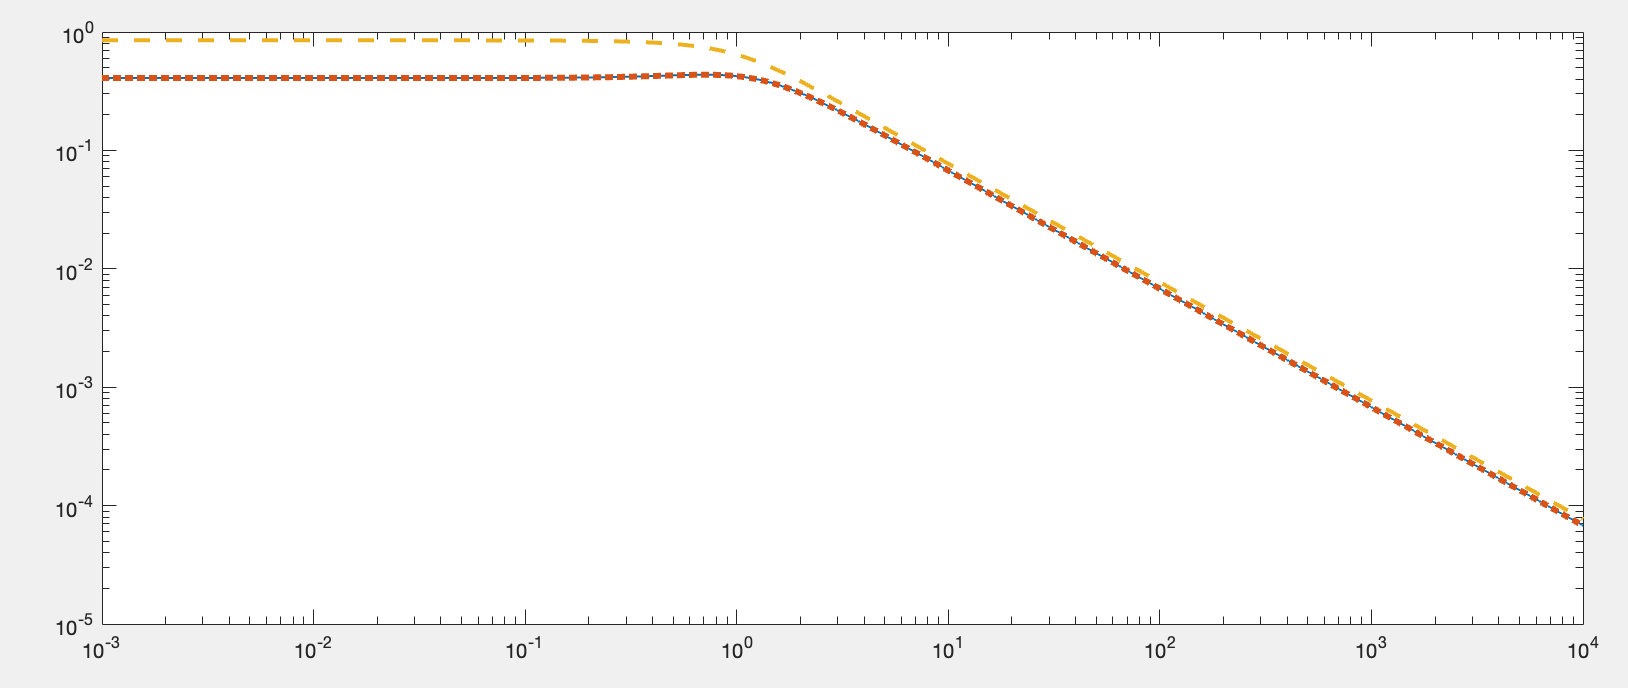
\includegraphics[width=1 \linewidth]{WorstCaseAmp}
			\caption{Dashed - worst case amplitude response, other two - a particular bode plot}
			\label{fig:worstcaseamp}
		\end{figure}
		
		
	\end{flushleft}
\end{frame}




\begin{frame}{Where are we}
	% \framesubtitle{O}
	\begin{flushleft}
		
		% TODO: \usepackage{graphicx} required
		\begin{figure}
			\centering
			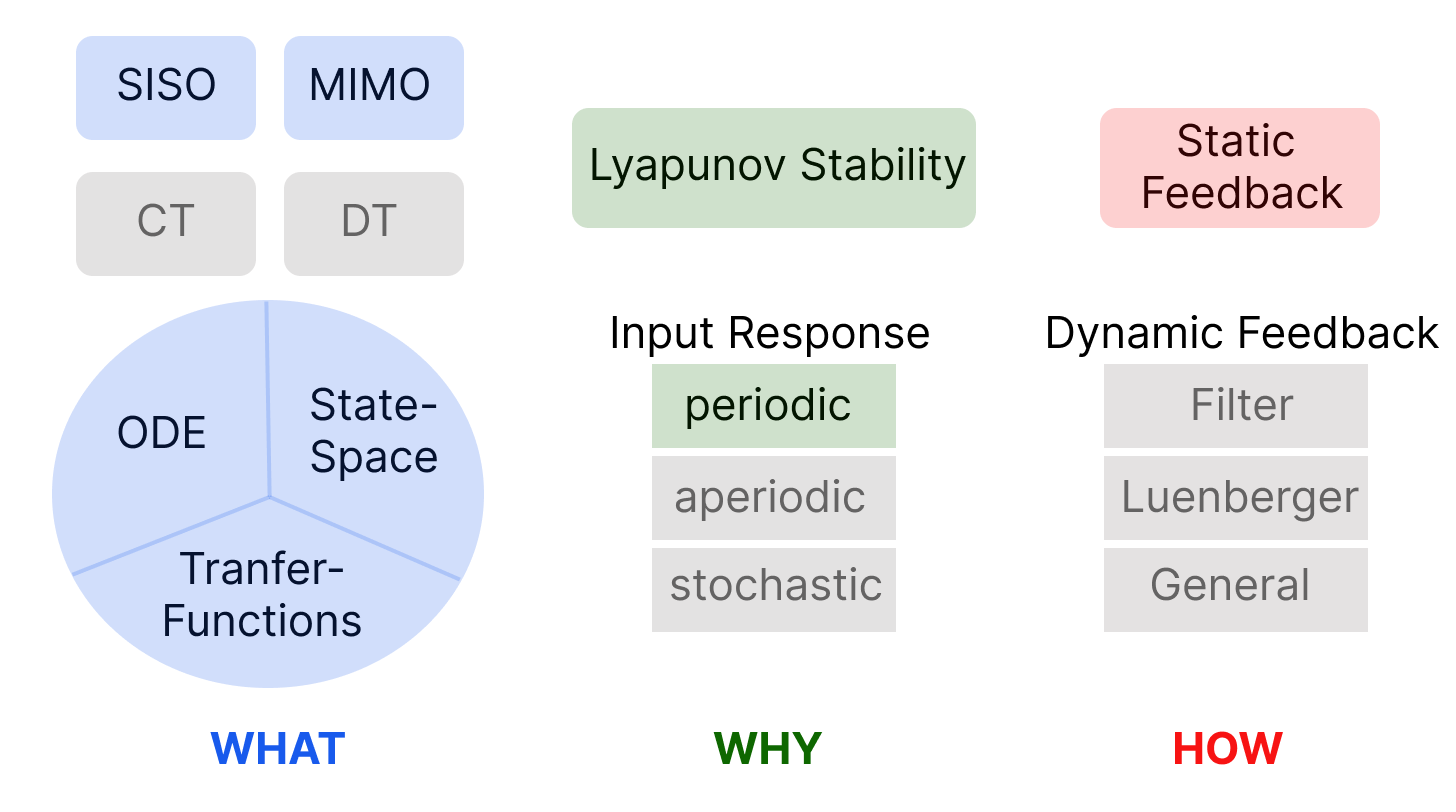
\includegraphics[width=1.0 \linewidth]{Scheme}
		\end{figure}
		
		
	\end{flushleft}
\end{frame}


\myqrframe






\end{document}
